\documentclass[11pt]{article}
\usepackage{acl}
\usepackage{times}
\usepackage{latexsym}
\usepackage[T1]{fontenc}
\usepackage[utf8]{inputenc}
\usepackage{microtype}
\usepackage{inconsolata}
\usepackage{graphicx}
\usepackage{amsmath}
\usepackage{amssymb}
\usepackage{booktabs}
\usepackage{tabularx}
\usepackage{xspace}
\usepackage{enumitem}
\usepackage{xcolor}
\usepackage{multirow}
\usepackage{tikz}
\usetikzlibrary{arrows.meta,positioning,shapes.geometric,fit,calc,backgrounds,decorations.pathreplacing}

\newcommand{\method}{\textsc{ExpertGym}\xspace}
\newcommand{\gdr}{\textsc{GDR}\xspace}
\newcommand{\grpo}{\textsc{GRPO}\xspace}
\newcommand{\opd}{\textsc{Recovery-OPD}\xspace}
\newcommand{\ret}{\textsc{Retention}\xspace}
\newcommand{\tool}{\textsc{Tool}\xspace}
\newcommand{\mem}{\textsc{Memory}\xspace}
\newcommand{\code}{\textsc{Code}\xspace}
\newcommand{\eqmerge}{\theta_{1/3}}
\newcommand{\TODO}{\textcolor{gray}{TBD}}
\newcommand{\creditcollapse}{\textit{Executable Credit Collapse}\xspace}
\newcommand{\vectorgym}{\textit{coefficient-space gym}\xspace}

\title{ExpertGym: Learning Agent Task-Vector Composition from Executable Feedback}
\author{Anonymous EMNLP Submission}

\begin{document}
\maketitle

\begin{abstract}
Task vectors provide a powerful prior for composing specialized models: each vector carries information about the expert's data distribution, trajectory style, and learned behavior.  However, agent task vectors cannot be composed reliably from weight-space geometry alone.  Tool use, memory update, and code generation succeed or fail only after executable rollouts, and the coefficient that preserves one agent behavior may suppress another.  We propose \method, a framework that turns frozen agent task-vector merging into a small, on-policy, executable-feedback-driven coefficient learning problem.  Starting from a symmetric one-third prior over \tool, \mem, and \code experts, \method learns only global, layer-wise, or module-wise coefficients over frozen deltas.  Calibration prompts are treated as probes rather than training examples: frontier prompts provide direction credit through group-relative optimization, same-prompt expert-recoverable failures provide recovery credit through verifier-grounded distillation, and stable successes provide boundary credit through retention.  This framing distinguishes \method from both geometric merging and imitation-based expert alignment: expert trajectories are not universal supervision, but recovery evidence that must be validated by executable rewards and non-regression guards.  We give a complete experimental framework for testing this claim, including state-distribution diagnostics, routed-versus-unrouted objectives, recovery-versus-imitation comparisons, coefficient granularity studies, and mixed-agent generalization.
\end{abstract}



\begin{figure*}[t]
\centering
\resizebox{0.94\linewidth}{!}{%
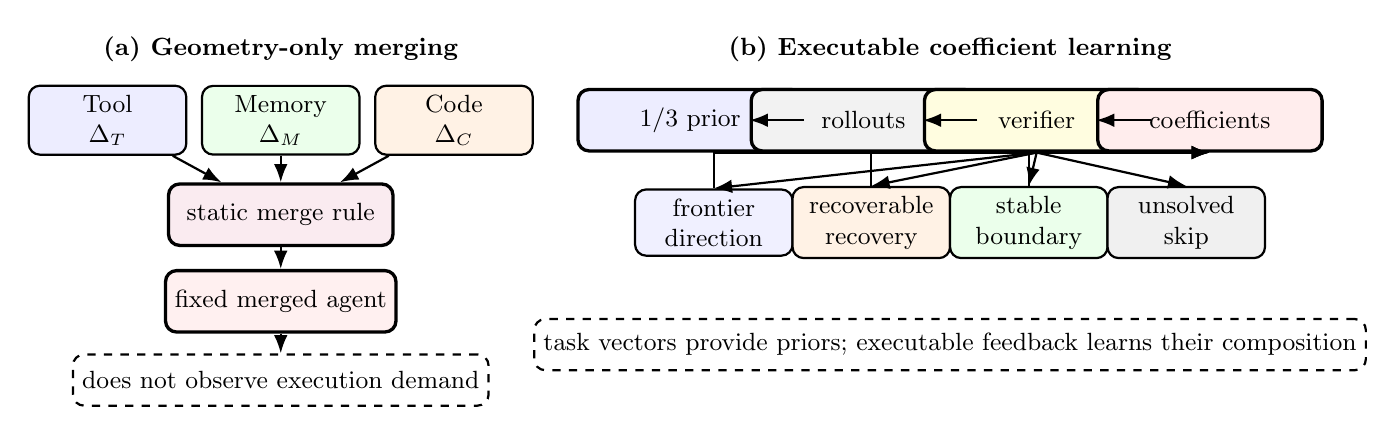
\begin{tikzpicture}[
  box/.style={draw, rounded corners, thick, align=center, minimum width=2.0cm, minimum height=0.68cm, fill=gray!8, font=\small},
  wide/.style={draw, rounded corners, very thick, align=center, minimum width=2.85cm, minimum height=0.78cm, font=\small},
  arr/.style={-Latex, thick},
  dashedbox/.style={draw, rounded corners, dashed, thick, align=center, font=\small, fill=white}
]
\node[font=\small\bfseries] at (2.2,3.55) {(a) Geometry-only merging};
\node[box, fill=blue!7] (gt) at (0,2.65) {Tool\\$\Delta_T$};
\node[box, fill=green!8] (gm) at (2.2,2.65) {Memory\\$\Delta_M$};
\node[box, fill=orange!10] (gc) at (4.4,2.65) {Code\\$\Delta_C$};
\node[wide, fill=purple!8] (gmerge) at (2.2,1.45) {static merge rule};
\node[wide, fill=red!6] (gagent) at (2.2,0.35) {fixed merged agent};
\node[dashedbox, minimum width=3.5cm, minimum height=0.65cm] (blind) at (2.2,-0.65) {does not observe execution demand};
\draw[arr] (gt) -- (gmerge); \draw[arr] (gm) -- (gmerge); \draw[arr] (gc) -- (gmerge); \draw[arr] (gmerge) -- (gagent); \draw[arr] (gagent) -- (blind);

\node[font=\small\bfseries] at (10.7,3.55) {(b) Executable coefficient learning};
\node[wide, fill=blue!7] (prior) at (7.4,2.65) {1/3 prior};
\node[wide, fill=gray!10] (roll) at (9.6,2.65) {rollouts};
\node[wide, fill=yellow!12] (ver) at (11.8,2.65) {verifier};
\node[wide, fill=red!7] (coef) at (14.0,2.65) {coefficients};
\draw[arr] (prior) -- (roll); \draw[arr] (roll) -- (ver); \draw[arr] (ver) -- (coef);
\node[box, fill=blue!6] (front) at (7.7,1.35) {frontier\\direction};
\node[box, fill=orange!10] (rec) at (9.7,1.35) {recoverable\\recovery};
\node[box, fill=green!8] (stable) at (11.7,1.35) {stable\\boundary};
\node[box, fill=gray!12] (unsolved) at (13.7,1.35) {unsolved\\skip};
\draw[arr] (ver.south) -- (front.north); \draw[arr] (ver.south) -- (rec.north); \draw[arr] (ver.south) -- (stable.north); \draw[arr] (ver.south) -- (unsolved.north);
\draw[arr] (front) |- (coef.south); \draw[arr] (rec) |- (coef.south); \draw[arr] (stable) |- (coef.south);
\node[dashedbox, minimum width=6.6cm, minimum height=0.65cm] at (10.7,-0.2) {task vectors provide priors; executable feedback learns their composition};
\end{tikzpicture}}
\caption{Central thesis.  Static merging can combine task vectors using weight-space structure, but agent composition additionally requires rollout-level information: which trajectories succeed, which expert can recover a failure, and which updates break already executable behavior.  \method keeps the task-vector prior frozen and learns only coefficients from executable feedback.}
\label{fig:thesis}
\end{figure*}

\section{Introduction}

Specialized LLM agents are increasingly trained for different executable capabilities: one agent is optimized for function calling, another for memory update, another for code generation, and another for reasoning or verification.  Serving a router over all experts is expensive, while fully retraining a generalist agent is slow and may erase expert-specific behavior.  Model merging offers an appealing middle ground: task vectors can be combined to produce a single deployed model without joint training or multi-expert inference \citep{wortsman2022model,ilharco2023editing}.

The usual model-merging story is geometric.  Given a base model and multiple experts, the method estimates how to add, trim, mask, align, or rescale task vectors so that parameter-side interference is reduced \citep{yadav2023ties,yu2023dare,deep2024della,gargiulo2025tsv,cheng2025wudi}.  This view is valuable, but it leaves out the central property of agents: success is only revealed by executing a trajectory.  A function-call model can have plausible logits while producing a non-parseable call; a memory model can answer a final question while corrupting intermediate state; a code model can imitate an expert trace but still fail unit tests.  Thus the right coefficient for composing agent task vectors cannot be inferred from weight-space geometry alone.

This paper studies the following question: \emph{How can we compose multiple agent task vectors when the right coefficient must be learned from executable trajectory feedback?}  Our answer is \method, a \vectorgym for frozen agent task vectors.  We begin from a symmetric one-third prior over \tool, \mem, and \code experts.  This start is not a naive accident: each task vector is a structured capability prior learned from an expert's data and trajectory distribution.  The goal is not to relearn the experts from scratch, but to use a small calibration panel to redistribute probability mass among existing expert directions.

A key distinction is that calibration examples are not ordinary supervised training data.  Because only coefficients are trainable while the base model and expert deltas remain frozen, calibration cannot freely memorize outputs.  Instead, prompts act as probes that reveal what kind of credit is available in the current merged policy.  Frontier prompts, where some rollouts succeed and others fail, provide direction credit for group-relative optimization.  Recoverable prompts, where the merge fails but a same-prompt expert succeeds, provide recovery credit.  Stable prompts, where the merge already succeeds, define a non-regression boundary.  Unsolved prompts, where neither merge nor experts succeed, should not update coefficients.

This framing also clarifies the relation to Expert Merging and imitation-based alignment.  Expert Merging learns layer-wise coefficients by aligning hidden states and logits of a merged model to expert behavior on unlabeled calibration data \citep{zhang2025expertmerging}.  Such alignment is useful, but it is not the same as executable success feedback.  In \method, expert trajectories are not universal targets.  They are used only when the current merged policy fails on the same prompt and an expert succeeds; the resulting recovery update is accepted only if executable rewards and retention guards show no cross-skill collapse.  This turns distillation from imitation into verifier-grounded recovery.

\paragraph{Contributions.}  This version of the paper makes four claims that are experimentally testable with the current code framework.
\begin{itemize}[leftmargin=*]
    \item We formulate \textbf{agent task-vector composition} as low-dimensional coefficient learning over frozen expert deltas from executable feedback.
    \item We identify \textbf{Executable Credit Collapse}: many agent calibration prompts are all-success, all-fail, or expert-recoverable, so they do not supply the same kind of coefficient credit.
    \item We propose \textbf{state-conditioned credit operators}: \grpo for frontier direction, same-prompt recovery distillation for suppressed expert priors, and retention for non-regression boundaries.
    \item We define a compact experimental program that separates geometry, imitation, recovery, and executable feedback, enabling rich diagnostics even before claiming state-of-the-art performance.
\end{itemize}

\section{Background and Positioning}

\paragraph{Task-vector priors.}  Let $\theta_0$ be a base model and $\theta_e$ be an expert model for skill $e\in\mathcal{E}$.  A task vector is $\Delta_e=\theta_e-\theta_0$.  For agents, $\Delta_e$ carries more than a label-specific preference: it encodes the expert's training data, decoding style, tool schema, memory protocol, and execution distribution.  This is why task-vector composition is attractive.  It preserves structure that would be costly to rediscover with full-parameter RL on a small calibration set.

\paragraph{Geometric merging.}  Static methods such as task arithmetic, TIES, DARE, DELLA, TSV, and WUDI improve how vectors are combined by handling sign conflict, redundancy, sparsity, singular structure, or interference \citep{ilharco2023editing,yadav2023ties,yu2023dare,deep2024della,gargiulo2025tsv,cheng2025wudi}.  These methods largely do not learn from the current merged agent's executable trajectories.  Our position is not that geometry is wrong; rather, geometry supplies a prior, but agent feedback supplies the missing demand signal.

\paragraph{Agent merging.}  Recent agent-oriented work argues that agent deltas are sparse, heterogeneous, and role-sensitive.  RAM studies reinforced agentic model merging and emphasizes behavior-knowledge preservation in RL-trained agents \citep{yuan2026ram}.  ARM proposes role-conditioned neuron transplantation for training-free generalist agent merging \citep{feng2026arm}.  These works motivate the same community problem: agent merging is not just static task merging.  \method is complementary because it focuses on verifier-side coefficient learning: how should a frozen composition move once we can execute the merged agent?

\paragraph{Imitation and on-policy distillation.}  On-policy distillation reduces mismatch by learning around outputs generated by the student policy rather than only teacher-forced data \citep{agarwal2024gkd}.  But in our setting, pure imitation is not enough.  Hidden-state or logit matching can align the merged model to experts without knowing whether the current merge actually failed, whether the expert was needed, or whether the update harms another agent behavior.  \method therefore treats distillation as a state-triggered recovery operator, not a general training objective.

\section{Problem Formulation}

\subsection{Coefficient Spaces}

The global composition is
\begin{equation}
    \theta(\alpha)=\theta_0+\sum_{e\in\mathcal{E}}\alpha_e\Delta_e.
\end{equation}
For three experts $\mathcal{E}=\{T,M,C\}$, the default initialization is
\begin{equation}
    \eqmerge=\theta_0+\frac{1}{3}(\Delta_T+\Delta_M+\Delta_C).
\end{equation}
A stable parameterization is common-plus-residual:
\begin{equation}
    \alpha_e=c+r_e,
\end{equation}
where $c$ controls shared expert strength and $r_e$ controls expert-specific residuals.  This makes training a controlled deviation from a symmetric prior rather than unconstrained coefficient search.

For fine-grained control, split parameters into groups $g\in\mathcal{G}$ such as layer bands or transformer modules:
\begin{equation}
    \theta(\alpha)=\theta_0+\sum_{e\in\mathcal{E}}\sum_{g\in\mathcal{G}}\alpha_{e,g}\Delta_{e,g}.
\end{equation}
The module-level setting supports micro-function control, e.g., attention routing versus FFN transformation.  It should be presented as a capacity study, not as the default main claim, unless experiments show clear non-regressive gains.

\subsection{Executable Feedback}

Given prompt $x$, the current merged policy samples $K$ trajectories
\begin{equation}
    y_1,\ldots,y_K\sim\pi_{\theta(\alpha)}(\cdot|x),\quad r_i=V(x,y_i),
\end{equation}
where $V$ is a task verifier.  \tool rewards parseable function calls with correct arguments, \mem rewards stateful memory update and final-answer correctness, and \code rewards code execution under official or generated tests.  These rewards are deliberately aligned with the original expert training environments when possible.

Define the empirical success rate $\hat p(x)$ and expert recoverability
\begin{equation}
    U(x)=\mathbb{I}\left[\exists e,\exists y_e^+\sim \pi_{\theta_e}(\cdot|x): V(x,y_e^+)>0\right].
\end{equation}
A prompt state is then assigned as follows:
\begin{equation}
S(x)=
\begin{cases}
\textsc{Frontier}, & 0<\hat p(x)<1,\\
\textsc{Recoverable}, & \hat p(x)=0 \text{ and } U(x)=1,\\
\textsc{Stable}, & \hat p(x)\approx1,\\
\textsc{Unsolved}, & \hat p(x)=0 \text{ and } U(x)=0.\\
\end{cases}
\end{equation}

\paragraph{Executable Credit Collapse.}  If most prompts are all-fail or all-success, then direct policy optimization over coefficients is compute-heavy but signal-poor.  If recoverable prompts are treated as ordinary imitation data, coefficients may drift toward one expert while hurting others.  If stable prompts are ignored, an apparent improvement can erase tool formats, memory state updates, or code executability.  We call this family of failures \creditcollapse.

\begin{figure}[t]
\centering
\resizebox{\columnwidth}{!}{%
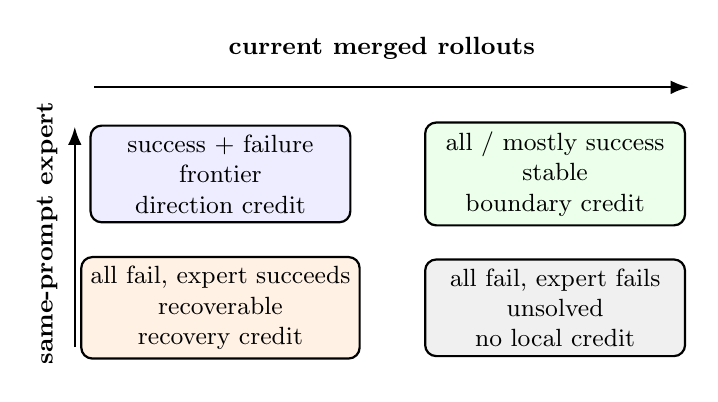
\begin{tikzpicture}[
  cell/.style={draw, rounded corners, thick, minimum width=3.3cm, minimum height=1.05cm, align=center, font=\small},
  arr/.style={-Latex, thick}
]
\node[font=\small\bfseries] at (2.05,2.35) {current merged rollouts};
\node[font=\small\bfseries, rotate=90] at (-2.2,0) {same-prompt expert};
\draw[arr] (-1.6,1.85) -- (5.95,1.85);
\draw[arr] (-1.85,-1.45) -- (-1.85,1.35);
\node[cell, fill=blue!7] at (0,0.75) {success + failure\\frontier\\direction credit};
\node[cell, fill=green!8] at (4.25,0.75) {all / mostly success\\stable\\boundary credit};
\node[cell, fill=orange!10] at (0,-0.95) {all fail, expert succeeds\\recoverable\\recovery credit};
\node[cell, fill=gray!12] at (4.25,-0.95) {all fail, expert fails\\unsolved\\no local credit};
\end{tikzpicture}}
\caption{Execution-state taxonomy.  The same calibration prompt can play different roles depending on current policy rollouts and same-prompt expert recovery.  This taxonomy is the bridge between theory and method.}
\label{fig:state-taxonomy}
\end{figure}

\section{Method: ExpertGym}

\method constructs a small on-policy calibration environment for coefficient learning.  It does not update base or expert weights.  It repeatedly samples rollouts from the current merged policy, verifies outcomes, routes prompts by state, applies the valid credit operator, and accepts only non-regressive coefficient updates.


\begin{figure*}[t]
\centering
\resizebox{0.96\linewidth}{!}{%
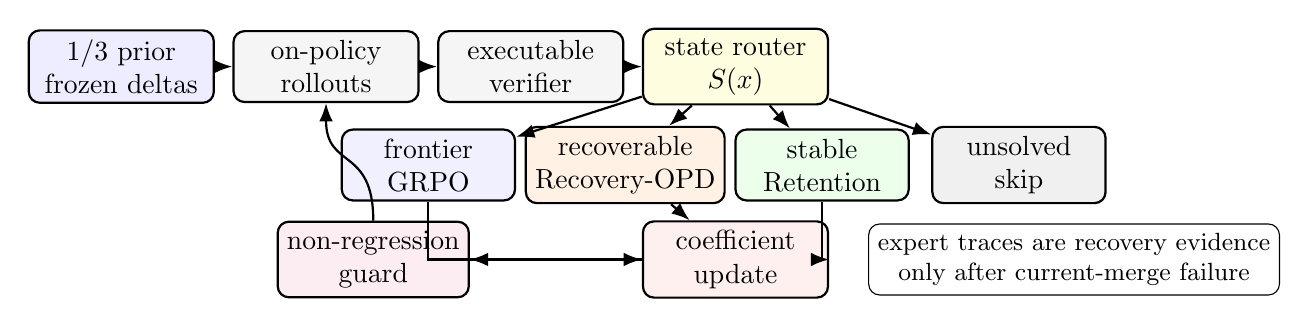
\begin{tikzpicture}[
  box/.style={draw, rounded corners, thick, align=center, minimum width=2.35cm, minimum height=0.78cm, fill=gray!8},
  op/.style={draw, rounded corners, thick, align=center, minimum width=2.2cm, minimum height=0.72cm},
  arr/.style={-Latex, thick},
  small/.style={font=\small}
]
\node[box, fill=blue!7] (init) at (0,2.6) {1/3 prior\\frozen deltas};
\node[box] (roll) at (2.6,2.6) {on-policy\\rollouts};
\node[box] (ver) at (5.2,2.6) {executable\\verifier};
\node[box, fill=yellow!12] (router) at (7.8,2.6) {state router\\$S(x)$};
\node[op, fill=blue!6] (g) at (3.9,1.35) {frontier\\GRPO};
\node[op, fill=orange!10] (d) at (6.4,1.35) {recoverable\\Recovery-OPD};
\node[op, fill=green!8] (r) at (8.9,1.35) {stable\\Retention};
\node[op, fill=gray!12] (s) at (11.4,1.35) {unsolved\\skip};
\node[box, fill=red!6] (upd) at (7.8,0.15) {coefficient\\update};
\node[box, fill=purple!7] (guard) at (3.2,0.15) {non-regression\\guard};
\node[draw, rounded corners, fill=white, align=center, small] (note) at (12.1,0.15) {expert traces are recovery evidence\\only after current-merge failure};
\draw[arr] (init) -- (roll); \draw[arr] (roll) -- (ver); \draw[arr] (ver) -- (router);
\draw[arr] (router) -- (g); \draw[arr] (router) -- (d); \draw[arr] (router) -- (r); \draw[arr] (router) -- (s);
\draw[arr] (g) |- (upd); \draw[arr] (d) -- (upd); \draw[arr] (r) |- (upd);
\draw[arr] (upd) -- (guard);
\draw[arr] (guard.north) .. controls +(up:0.95cm) and +(down:0.85cm) .. (roll.south);
\end{tikzpicture}}
\caption{\method training loop.  The algorithm is a coefficient-space agent gym: a small calibration set creates real rollouts, verifiers assign execution states, and each state selects the valid credit operator.}
\label{fig:loop}
\end{figure*}

\subsection{Frontier Direction: GRPO over Coefficients}

For frontier prompts, rewards vary among sampled trajectories.  We use a group-relative objective inspired by GRPO \citep{shao2024deepseekmath}.  With normalized advantage
\begin{equation}
    \hat A_i=\frac{r_i-\bar r}{\mathrm{std}(r_1,\ldots,r_K)+\epsilon},
\end{equation}
we update coefficients with a clipped objective
\begin{equation}
\mathcal{L}_{G}=-\mathbb{E}\left[\min\left(\rho_i\hat A_i,\mathrm{clip}(\rho_i,1-\epsilon_c,1+\epsilon_c)\hat A_i\right)\right],
\end{equation}
where $\rho_i$ is computed between current and old coefficients.  This term is only valid where reward variance exists.  The paper should not claim that GRPO solves all coefficient learning; it supplies direction credit on the frontier subset.

\subsection{Recoverable Failures: Distillation as Verifier-Grounded Recovery}

For recoverable prompts, current rollouts fail but a same-prompt expert succeeds.  Let $y_e^+$ denote that successful expert trajectory.  The recovery loss is
\begin{equation}
    \mathcal{L}_{D}= -\mathbb{E}_{(x,e,y_e^+)} w_{x,e}\frac{1}{|y_e^+|^{\gamma}}\log \pi_{\theta(\alpha)}(y_e^+|x).
\end{equation}
This is deliberately not generic imitation.  The trigger requires current failure and expert success on the same prompt.  The weight $w_{x,e}$ can incorporate expert margin, task balance, and gradient agreement with frontier updates.  Candidate updates induced by $\mathcal{L}_D$ must pass executable validation before being kept.

\paragraph{Why this is different from Expert Merging.}  Expert Merging aligns hidden states and logits on unlabeled calibration data to learn layer-wise coefficients \citep{zhang2025expertmerging}.  Our recovery objective is narrower and more agentic: it asks whether an expert trajectory recovers a concrete failure of the current merge, and whether the resulting coefficient movement improves executable outcomes without breaking other skills.  This distinction should be made explicit in the experiments through imitation-only and hidden/logit-alignment baselines.

\subsection{Stable Successes: Retention as Boundary Credit}

Stable prompts define safe regions.  Let $y^+$ be a successful response from the reference or accepted merged policy.  Retention uses
\begin{equation}
    \mathcal{L}_{R}= -\mathbb{E}_{(x,y^+)\in\mathcal{G}}\log \pi_{\theta(\alpha)}(y^+|x).
\end{equation}
This term is not expected to discover new capability.  Its role is to mark a boundary: updates should not erase parseability, memory update consistency, or code execution patterns that are already solved.  This framing makes retention a necessary guard rather than an arbitrary regularizer.

\subsection{Credit Normalization and Guarded Update}

The total objective is
\begin{equation}
    \mathcal{L}=\lambda_G\mathcal{L}_{G}+\lambda_D\mathcal{L}_{D}+\lambda_R\mathcal{L}_{R}+\lambda_2\|\alpha-\alpha_{1/3}\|_2^2.
\end{equation}
Because recoverable prompts can be numerous early in training, we recommend gradient-budget balancing:
\begin{equation}
    \lambda_j\leftarrow\mathrm{clip}\left(\frac{b_j}{\mathrm{EMA}(\|\nabla_\alpha\mathcal{L}_j\|)+\epsilon},\lambda_j^{\min},\lambda_j^{\max}\right),
\end{equation}
for $j\in\{G,D,R\}$.  After each interval, a candidate coefficient update is evaluated on a held-out guard set.  It is accepted only if average reward improves or remains stable and worst-task regression is below a threshold $\delta$.

\begin{table}[t]
\centering
\small
\setlength{\tabcolsep}{3pt}
\resizebox{\columnwidth}{!}{%
\begin{tabular}{llll}
\toprule
State & Observable condition & Credit & Operator \\
\midrule
Frontier & mixed rollout rewards & direction & GRPO \\
Recoverable & merge fails, expert succeeds & recovery & same-prompt OPD \\
Stable & merge already succeeds & boundary & retention \\
Unsolved & merge and experts fail & none & skip / data acquisition \\
\bottomrule
\end{tabular}}
\caption{Core method as an evidence-to-objective map.  This table should remain central in the final paper: it makes the loss design look inevitable rather than heuristic.}
\label{tab:evidence-map}
\end{table}

\section{Experiments}

The experimental program is designed to support the story before chasing leaderboard claims.  The key is to show that \method solves a problem that geometric merging and imitation-only alignment do not address.

\subsection{Benchmarks and Metrics}

\tool uses function-call exactness, argument correctness, parseability, and schema validity.  \mem uses multi-turn memory update with final-answer EM/F1.  \code uses Pass@1, any-pass@K reachability, and best-of-$K$ selection accuracy.  Main tables should report average score, worst-task drop relative to $\eqmerge$, and collapse count.  A method that increases average while breaking one skill should not be considered successful.

\subsection{E1: Task Vectors Contain Structured Priors}

This experiment establishes why the one-third prior is meaningful.  It compares base, single experts, and $\eqmerge$.  The expected conclusion is not that $\eqmerge$ is optimal, but that it is stronger than base and exposes real multi-skill behavior while still showing composition trade-offs.

\begin{table}[t]
\centering
\small
\setlength{\tabcolsep}{4pt}
\begin{tabular}{lccccc}
\toprule
Model & Tool & Memory & Code & Avg. & Worst drop \\
\midrule
Base & \TODO & \TODO & \TODO & \TODO & -- \\
Tool expert & \TODO & \TODO & \TODO & \TODO & \TODO \\
Memory expert & \TODO & \TODO & \TODO & \TODO & \TODO \\
Code expert & \TODO & \TODO & \TODO & \TODO & \TODO \\
Equal-prior $\eqmerge$ & \TODO & \TODO & \TODO & \TODO & ref. \\
\bottomrule
\end{tabular}
\caption{Task-vector prior table.  This table should show that expert deltas contain useful skill priors, while equal-prior composition still leaves room for feedback-conditioned coefficient learning.}
\label{tab:priors}
\end{table}

\subsection{E2: Geometry Cannot Infer Executable Demand}

This experiment compares static geometric merging to executable-feedback-conditioned learning.  Baselines should include task arithmetic, best static scale sweep, TIES, DARE+TA, WUDI/TSV-style structure-aware merging, RAM/ARM-style agent merging if available, and Expert Merging-style coefficient alignment.  The current filled numbers report Tool mean, Memory F1, and Code Pass@1/Acc. under the same Eval6 harness; average is the mean of those three columns.

\begin{table*}[t]
\centering
\small
\setlength{\tabcolsep}{3.2pt}
\begin{tabular}{lcccccccc}
\toprule
Method & Learns? & Exec. feedback? & Tool & Memory & Code & Avg. & Worst drop & Collapse \\
\midrule
TA $1/3$ & no & no & 0.785 & 0.646 & 0.341 & 0.591 & ref. & 0 \\
TA $0.75$ & no & no & 0.785 & 0.759 & 0.349 & 0.631 & 0.000 & 0 \\
TIES & no & no & 0.764 & 0.636 & 0.336 & 0.579 & -0.021 & 2 \\
DARE+TA & no & no & 0.795 & 0.690 & 0.337 & 0.607 & -0.004 & 0 \\
DARE+TIES & no & no & 0.795 & 0.689 & 0.343 & 0.609 & 0.002 & 0 \\
AdaMerging & coeff. & entropy & 0.784 & 0.668 & 0.341 & 0.597 & -0.001 & 0 \\
Mixture GRPO & full & yes & 0.782 & 0.664 & 0.338 & 0.595 & -0.003 & 0 \\
\method global 3 & coeff. & yes & 0.792 & 0.666 & 0.342 & 0.600 & 0.001 & 0 \\
\method common+res. & coeff. & yes & 0.786 & 0.690 & 0.337 & 0.604 & -0.004 & 0 \\
\bottomrule
\end{tabular}
\caption{Main comparison snapshot.  Static scale selection is a strong baseline on Memory, while executable-feedback coefficient learning gives non-regressive movement from the equal-prior start.  The current numbers support a cautious claim about learnable composition rather than a SOTA claim.}
\label{tab:main}
\end{table*}

\subsection{E3: Calibration State Distribution}

This table is the empirical basis for the paper's insight.  We roll out $\eqmerge$ on 96 balanced evaluation-targeted calibration prompts with $K=8$ samples and classify each prompt by current rollout outcomes and same-prompt expert recoverability.

\begin{table}[t]
\centering
\small
\setlength{\tabcolsep}{4pt}
\begin{tabular}{lccccc}
\toprule
Skill & Frontier & Recover. & Stable & Unsolved & Std. \\
\midrule
Tool & 14 & 1 & 10 & 7 & 0.243 \\
Memory & 28 & 3 & 0 & 1 & 0.389 \\
Code & 12 & 6 & 2 & 12 & 0.197 \\
All & 54 & 10 & 12 & 20 & 0.276 \\
\bottomrule
\end{tabular}
\caption{Executable state distribution at the equal-prior start.  Frontier prompts justify GRPO, recoverable prompts justify same-prompt recovery-OPD, and stable prompts justify retention.  Code has the largest unsolved mass, which explains why Code improvement remains the hardest held-out dimension.}
\label{tab:states}
\end{table}

\subsection{E4: Routing Matters More than Loss Mixing}

\begin{table}[t]
\centering
\small
\setlength{\tabcolsep}{3.2pt}
\resizebox{\columnwidth}{!}{%
\begin{tabular}{lcccccc}
\toprule
Method & GRPO & OPD & Ret. & Routed & Avg. & Drop \\
\midrule
GRPO only & yes & no & no & partial & \TODO & \TODO \\
OPD only & no & yes & no & partial & \TODO & \TODO \\
Retention only & no & no & yes & partial & \TODO & \TODO \\
Unrouted weighted sum & yes & yes & yes & no & \TODO & \TODO \\
Random routing & yes & yes & yes & random & \TODO & \TODO \\
\method & yes & yes & yes & state & \TODO & \TODO \\
\bottomrule
\end{tabular}}
\caption{Loss and routing ablation.  The crucial result is \method beating the unrouted weighted sum, which would show that the contribution is execution-state credit assignment rather than a tuned loss mixture.}
\label{tab:ablation}
\end{table}

\subsection{E5: Recovery Is Not Imitation}

This is the most important defensive experiment.  It should compare generic expert imitation, Expert Merging-style hidden/logit alignment, offline expert traces, same-prompt recoverable OPD, and verifier-guarded recovery.

\begin{table*}[t]
\centering
\small
\setlength{\tabcolsep}{3.2pt}
\begin{tabular}{lcccccccc}
\toprule
Method & Trigger & Signal & Verifier guard & Tool & Memory & Code & Avg. & Drop \\
\midrule
Offline trace distill & always & expert traj. & no & \TODO & \TODO & \TODO & \TODO & \TODO \\
Logit imitation & always & expert logits & no & \TODO & \TODO & \TODO & \TODO & \TODO \\
Hidden/logit align & always & expert states & no & \TODO & \TODO & \TODO & \TODO & \TODO \\
Same-prompt OPD & merge all-fail & expert success & no & \TODO & \TODO & \TODO & \TODO & \TODO \\
Same-prompt OPD + guard & merge all-fail & expert success & yes & \TODO & \TODO & \TODO & \TODO & \TODO \\
Full \method & state-conditioned & mixed credit & yes & \TODO & \TODO & \TODO & \TODO & \TODO \\
\bottomrule
\end{tabular}
\caption{Recovery versus imitation.  This experiment directly addresses the risk that distillation looks like ordinary imitation.  The target result is not necessarily that recovery always gives the largest raw gain, but that it gives safer executable improvement under worst-task non-regression.}
\label{tab:imitation}
\end{table*}

\subsection{E6: Code Planning Diagnostic}

Because code success depends on planning and execution, imitation-only metrics are insufficient.  Split code into reachability and selection.

\begin{table}[t]
\centering
\small
\setlength{\tabcolsep}{3pt}
\resizebox{\columnwidth}{!}{%
\begin{tabular}{lcccc}
\toprule
Method & Any-pass@K & BoN select & Pass@1 & Main failure \\
\midrule
$\eqmerge$ & \TODO & \TODO & \TODO & \TODO \\
OPD only & \TODO & \TODO & \TODO & \TODO \\
GRPO only & \TODO & \TODO & \TODO & \TODO \\
Full \method & \TODO & \TODO & \TODO & \TODO \\
\bottomrule
\end{tabular}}
\caption{Code diagnostic.  Recovery may improve reachability by moving the merge toward expert-like correct trajectories, while executable feedback is needed to validate planning-sensitive outcomes.}
\label{tab:code-diagnostic}
\end{table}

\subsection{E7: Coefficient Granularity and Overfit}

The module-level story is attractive but must be handled carefully.  The right claim is that finer coefficient spaces provide more local repair directions, but only if retention and held-out validation prevent overfitting.

\begin{table}[t]
\centering
\small
\setlength{\tabcolsep}{3pt}
\resizebox{\columnwidth}{!}{%
\begin{tabular}{lcccccc}
\toprule
Space & Params & Tool & Mem. & Code & Avg. & Gap \\
\midrule
Global 3 & 3 & \TODO & \TODO & \TODO & \TODO & \TODO \\
Common+residual & 4 & \TODO & \TODO & \TODO & \TODO & \TODO \\
Layer-wise & \TODO & \TODO & \TODO & \TODO & \TODO & \TODO \\
Module-wise & 588 & \TODO & \TODO & \TODO & \TODO & \TODO \\
Module + guard & 588 & \TODO & \TODO & \TODO & \TODO & \TODO \\
\bottomrule
\end{tabular}}
\caption{Coefficient capacity ladder.  If global coefficients already capture most gains, the paper can argue that task-vector priors are strong.  If module gates improve results, the paper can argue for localized micro-function repair.}
\label{tab:capacity}
\end{table}

\subsection{E8: Mixed-Agent Generalization}

To make the paper more than a benchmark-specific merge, add a small mixed-agent evaluation set: Tool+Memory, Memory+Code, Tool+Code, and Tool+Memory+Code prompts.  These prompts test whether task vectors can produce combination generalization when executable feedback learns the composition.

\begin{table}[t]
\centering
\small
\setlength{\tabcolsep}{3pt}
\resizebox{\columnwidth}{!}{%
\begin{tabular}{lccccc}
\toprule
Method & T+M & M+C & T+C & T+M+C & Avg. \\
\midrule
$\eqmerge$ & \TODO & \TODO & \TODO & \TODO & \TODO \\
Static best & \TODO & \TODO & \TODO & \TODO & \TODO \\
Imitation-only & \TODO & \TODO & \TODO & \TODO & \TODO \\
Full \method & \TODO & \TODO & \TODO & \TODO & \TODO \\
\bottomrule
\end{tabular}}
\caption{Mixed-agent generalization.  This is the most attractive optional experiment: it tests whether coefficient learning unlocks behavior combinations not directly represented by any single expert.}
\label{tab:mixed}
\end{table}

\section{Analysis Figures to Fill}

\begin{figure*}[t]
\centering
\resizebox{0.96\linewidth}{!}{%
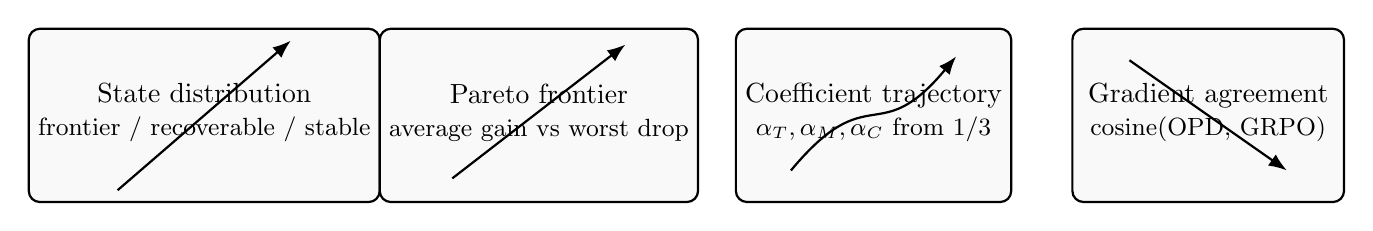
\begin{tikzpicture}[
  panel/.style={draw, rounded corners, thick, minimum width=3.45cm, minimum height=2.2cm, align=center, fill=gray!5},
  arr/.style={-Latex, thick},
  small/.style={font=\small}
]
\node[panel] (p1) at (0,0) {State distribution\\\vspace{0.2em}\small frontier / recoverable / stable};
\node[panel] (p2) at (4.25,0) {Pareto frontier\\\vspace{0.2em}\small average gain vs worst drop};
\node[panel] (p3) at (8.5,0) {Coefficient trajectory\\\vspace{0.2em}\small $\alpha_T,\alpha_M,\alpha_C$ from 1/3};
\node[panel] (p4) at (12.75,0) {Gradient agreement\\\vspace{0.2em}\small cosine(OPD, GRPO)};
\draw[arr] (-1.1,-0.95) -- (1.1,0.95);
\draw[arr] (3.15,-0.8) -- (5.35,0.9);
\draw[arr] (7.45,-0.7) .. controls +(1,1.2) and +(-1,-1.2) .. (9.55,0.75);
\draw[arr] (11.75,0.7) -- (13.75,-0.7);
\end{tikzpicture}}
\caption{Analysis dashboard template.  These four plots make the paper visually rich without overclaiming: they show where signal comes from, how non-regression is enforced, how coefficients move, and whether recovery and direction gradients conflict.}
\label{fig:dashboard}
\end{figure*}

\paragraph{Expected useful findings.}  Even if final scores are modest, the paper can be strong if it shows: (i) frontier signal is sparse, explaining why pure GRPO is slow; (ii) recoverable prompts exist, explaining why recovery is needed; (iii) generic imitation creates cross-task regression, while same-prompt recovery plus guard is safer; and (iv) coefficient updates reveal interpretable skill trade-offs.

\section{Possible Solutions for Current Bottlenecks}

\paragraph{If OPD dominates coefficient movement.}  Do not hide it.  Reframe OPD as early-phase recovery and report its gradient share.  Add a schedule that decays recovery weight as frontier prompts increase.  A useful diagnostic is the percentage of recovered prompts that later become frontier or stable under the updated merge.

\paragraph{If GRPO is weak.}  Restrict GRPO claims to frontier prompts.  Improve its signal by frontier oversampling, reward shaping from verifier components, and per-task advantage normalization.  For code, reward shaping can separate parse success, compilation, unit-test pass, and hidden-test pass.

\paragraph{If retention only prevents collapse.}  That is the intended role.  Present retention sweeps as a Pareto boundary: higher retention should reduce worst-task drop while potentially limiting gains.  The figure should show a trade-off curve, not a single magic coefficient.

\paragraph{If module gates overfit.}  Use held-out calibration guards and coefficient sparsity.  Module-level results can be framed as analysis unless they clearly improve non-regressive metrics.

\paragraph{If Expert Merging is a strong baseline.}  That is useful.  Position \method as adding executable recovery and non-regression guards on top of coefficient learning.  The most important direct comparison is hidden/logit alignment versus same-prompt recovery under executable metrics.

\section{Related Work}

\paragraph{Model merging and task vectors.}  Model soups showed that weight averaging can improve accuracy without additional inference cost \citep{wortsman2022model}.  Task arithmetic framed fine-tuning deltas as editable capability vectors \citep{ilharco2023editing}.  TIES, DARE, DELLA, TSV, and WUDI reduce interference through sign resolution, sparsification, sampling, singular structure, or data-free vector guidance \citep{yadav2023ties,yu2023dare,deep2024della,gargiulo2025tsv,cheng2025wudi}.  \method keeps this prior but learns how to activate it from executable rollouts.

\paragraph{Agent merging.}  RAM and ARM extend merging concerns to reinforced or interactive agents, emphasizing sparse behavior knowledge, role-conditioned activations, and training-free integration \citep{yuan2026ram,feng2026arm}.  \method is complementary: instead of deciding which neurons to transplant, it asks how frozen agent vectors should be scaled after observing actual execution outcomes.

\paragraph{Expert alignment and distillation.}  Expert Merging learns layer-wise coefficients using hidden-state and logit alignment on unlabeled calibration data \citep{zhang2025expertmerging}.  On-policy distillation addresses distribution mismatch by learning from student-generated behavior \citep{agarwal2024gkd}.  We use expert behavior more narrowly: same-prompt expert success is recovery evidence for a current merge failure, not universal supervision.

\paragraph{Executable feedback.}  Agent benchmarks such as BFCL, memory-grounded QA, LiveCodeBench, and code-unit-test reinforcement show why final executable reward differs from static next-token similarity \citep{patil2025bfcl,yang2018hotpotqa,jain2025livecodebench,wang2025cure}.  \method uses this property as the core learning signal for coefficient composition.

\section{Conclusion}

\method reframes agent merging as executable-feedback-driven coefficient learning.  Task vectors provide structured priors; executable trajectories tell us how to compose them.  The paper's main novelty is not a larger coefficient space or a stronger imitation loss, but a state-conditioned calibration framework that separates direction, recovery, and boundary credit.  This gives a plausible and defensible path from current experiments to a review-ready EMNLP paper: show that geometry alone misses rollout demand, imitation alone lacks success-grounded credit, and small coefficient-space learning can improve or stabilize agent task-vector composition under non-regression constraints.

\bibliography{references}

\appendix

\section{Agent Group Synthesis}

\paragraph{Strategist.}  The paper must sell a problem, not a training recipe.  The center sentence is: task vectors provide the prior; executable feedback learns the composition.

\paragraph{Method architect.}  Distillation is the weak point if presented as imitation.  It becomes novel only when triggered by current-merge failure, same-prompt expert success, and verifier acceptance.

\paragraph{Experiment designer.}  The first result should be state distribution, not final benchmark score.  The key ablation is state-routed objective versus unrouted loss mixture.

\paragraph{Skeptical reviewer.}  Do not claim SOTA before RAM, ARM, Expert Merging, and geometric baselines are implemented on the same suite.  The safer claim is non-regressive improvement and diagnostic insight.

\section{Minimum Run Plan}

\begin{enumerate}[leftmargin=*]
    \item Roll out $\eqmerge$ on 100--150 balanced calibration prompts with $K=8$ or $K=16$ samples.  Fill Table~\ref{tab:states}.
    \item Run global 3 and common+residual 4 coefficient spaces before module-level gates.
    \item Compare GRPO-only, OPD-only, retention-only, full routed \method, unrouted sum, random routing, and task-only routing.
    \item Compare offline trace distillation, logit imitation, hidden/logit Expert-Merging-style alignment, same-prompt OPD, and verifier-guarded recovery.
    \item For code, report any-pass@K, BoN selection, and Pass@1 rather than only aggregate accuracy.
    \item Add mixed-agent prompts after the single-skill loop works.  This is the highest-impact optional experiment.
\end{enumerate}

\section{Claim Ladder}

\paragraph{Safe claim.}  \method formulates agent task-vector composition as executable-feedback-driven coefficient learning and provides diagnostics that static geometric merging lacks.

\paragraph{Medium claim.}  State routing is necessary because frontier, recoverable, and stable prompts provide different valid credit types.

\paragraph{Strong claim.}  \method improves over geometric and imitation-only merging under non-regression across Tool, Memory, and Code.

\paragraph{Do not claim yet.}  State-of-the-art agent merging, unless all strong baselines are run on the same held-out suite.

\end{document}
